\begin{comment}
------------------------------------------------------------------------------------------
\end{comment}
\chapter{Grundlagen}


\begin{comment}
------------------------------------------------------------------------------------------
- https://de.wikipedia.org/wiki/Fading_(Elektrotechnik)
\end{comment}
\section{Verfahren für die Entfernungsbestimmung}

Bei der \textit{Triangulation} werden die Winkel zwischen mehreren Referenzpunkten bestimmt und dann die dazu gehörige Entfernung mittels trigonometrischer Funktionen berechnet. Dieses Verfahren ist auch unter den Namen \Gls{aoa} bzw. \Gls{doa} bekannt. Um eine genau Ortsbestimmung durchzuführen müssen die Winkel sehr genau bestimmt werden. Um das zu bewerkstelligen werden im Empfänger mehrere Antennen zu einem Feld (engl. Antenna Array) zusammengefasst. Jedoch ist diese Konstruktion sehr teuer und empfindlich für Mehrwegeempfang (engl. Multipath) bzw. Signalabschattungen. \cite{gezici2005localization, liu2007survey, decawave2014rtls}

Im Gegensatz dazu werden bei der \textit{Trilateration} die Entfernungen zwischen mehreren Referenzpunkten betrachtet. Es werden dabei die Verfahren \Gls{toa} und \Gls{tdoa} unterschieden.
Bei dem \Gls{toa}--Verfahren wird zuerst die Zeitdifferenz zwischen dem Senden und Empfangen eines Funksignals berechnet. Mittels der Signallaufzeit (engl. \acrfull{tof}) und der Ausbreitungsgeschwindigkeit des Funksignals kann die Entfernung berechnet werden. Die Ortsbestimmung erfolgt dann über die Schnittpunkte von drei Kreisen (2D) bzw. vier Kugeln (3D) miteinander. Um dieses Verfahren anwenden zu können, ist es erforderlich das das Funksignal mit einem Zeitstempel des Startzeitpunktes versehen ist. Daraus folgt aber auch, das die Zeit zwischen Sender und Empfänger sehr genau synchronisiert werden müssen um den Fehler möglich klein zu halten.
Bei dem \Gls{tdoa}--Verfahren werden die Zeitdifferenz zwischen dem Empfang des Funksignals an mehreren Empfängern ausgewertet. Dies hat den großen Vorteil das nur noch die Zeit zwischen den Empfängern synchronisiert werden muss. \cite{zekavat2011handbook, decawave2014rtls}

Neben der \textit{Triangulation} und \textit{Trilateration} besteht auch die Möglichkeit auf Grund der empfangenen Signalstärke (engl. \acrfull{ss_radio}, \acrfull{rss} oder auch \acrfull{rssi}) Rückschlüsse über die Entfernung zu ziehen. Dazu muss die ursprüngliche Signalstärke und die Ausbreitungscharakteristik der elektromagnetischen Welle in der spezifischen Umgebung bekannt sein. \cite{gezici2005localization, decawave2014rtls}

In den nächsten zwei Abschnitten werden die \textit{DecaWave} Entfernungsmessverfahren vorgestellt. Diese haben den Vorteil, dass keine Synchronisierung der Zeit zwischen Sender und Empfänger notwendig ist. Weiterhin besitzen die \textit{DecaWave} \Gls{uwbt} zwei Eigenschaften die die Entfernungsmessung ideal ergänzt. Zum einen wird jede erhaltene Nachricht mit einem lokalen Zeitstempel versehen, der über eine minimale Auflösung von ungefähr \SI{15.65}{\pico\second} verfügt. Hiermit wäre eine theoretische Ortsauflösung von ungefähr \SI{5}{\milli\metre} möglich. Des Weiteren ist es möglich, den Sendezeitpunkt einer Nachricht in die Zukunft zu legen. Damit lässt sich die Zeitspanne zwischen dem Empfang und der Antwort auf eine Nachricht im Voraus berechnen. Die Zeitspanne kann dann der Antwortnachricht als Nutzlast mitgegeben werden, um beim Empfänger die Umlaufzeit zu berechnen.


\begin{comment}
------------------------------------------------------------------------------------------
- Wie lange dauert es bis eine Nachricht ausgetauscht worden ist?
	- Beispiel mit einer konkreten Entfernung?
	
- Wie schnell drifted ein Quarz in einem µc?
	- What is the ppm in the crystal oscillator?
	- https://electronics.stackexchange.com/questions/15851/what-is-the-ppm-in-the-crystal-oscillator
	- In the 1930s, such precise time measurements simply weren't possible; a clock of the required accuracy was difficult enough to build in fixed form, let alone portable. A crystal oscillator, for instance, drifts about 1 to 2 seconds in a month, or 1.4x10−3 seconds an hour.[1] This may sound small, but as light travels 3x108 m/s, this represents a drift of 400 m per hour. Only a few hours of flight time would render such a system unusable, a situation that remained in force until the introduction of commercial atomic clocks in the 1960s.
	- Clock accuracy in ppm
	- http://www.best-microcontroller-projects.com/ppm.html
	

\end{comment}
\subsection{Single-sided Two-way Ranging}

Das einfachste Verfahren, um aus der Umlaufzeit die Entfernung abzuschätzen, ist das \Gls{sstwr}--Verfahren. Dabei sendet der \Gls{tag} eine Nachricht an den \Gls{anchor} und wartet ab, bis eine entsprechende Antwortnachricht eintrifft. Beide Module erhalten einen Zeitstempel für den Versand und Empfang von Nachrichten. Aus diesen kann dann die Antwort-- ($T_{reply}$) und Umlaufzeit ($T_{round}$) berechnet werden, siehe \figurename~\ref{fig:single_sided_two_way_ranging}. \cite{decawave2015twr, decawave2016dw1kusermanual}

\begin{figure}[ht]
	\centering
	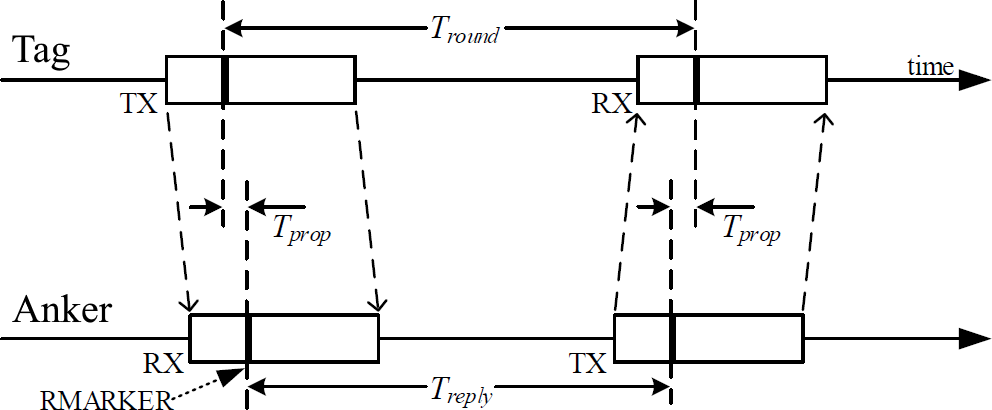
\includegraphics[width=0.75\linewidth]{single_sided_two_way_ranging}
	\caption{Ablauf des \acrlong{sstwr}.}
	\source{\citetitle{decawave2016dw1kusermanual} \cite{decawave2016dw1kusermanual}}
	\label{fig:single_sided_two_way_ranging}
\end{figure}

Die ungefähre \Gls{tof}--Zeitspanne ergibt sich aus der folgenden Gleichung:

\[T_{prop}=\frac{1}{2}\left(T_{round}-T_{reply}\right)\]

Damit der \Gls{tag} die \Gls{tof}--Zeitspanne berechnen kann, benötigt er die $T_{reply}$--Zeitspanne. Zu diesem Problem gibt es mehrere Lösungen. Die einfachste Lösung ist eine feste Antwortzeit die jedem Modul bekannt ist. Alternativ kann der \Gls{anchor} in der Antwortnachricht seine individuelle Antwortzeit übermitteln. Oder der \Gls{tag} übermittelt dem \Gls{anchor} mit der initialen Nachricht wie lange der \Gls{anchor} warten muss bis er die Antwortnachricht verschickt. Hierbei muss die Zeitspanne groß genug gewählt sein, um den \Gls{anchor} die Möglichkeit zur Antwort zu lassen. Je nach Anforderung wird eine der vorherigen Methoden verwendet.

Der Nachteil bei diesem Verfahren besteht in dem Fehler der von der Antwortzeit abhängt. Bei Module verwenden zur Berechnung von $T_{round}$ und $T_{reply}$ ihre lokalen Zeitgeber. Beide Zeitgeber haben einen Offsetfehler $e_{A}$ und $e_{B}$ der von der Nennfrequenz abweicht. Die daraus abgeleitete \Gls{tof}--Zeitschätzung hat damit einen Fehler der mit der Antwortzeit wächst:

\[error\approx\frac{1}{2}\left(e_B-e_A\right)\times T_{reply}\]


\begin{comment}
------------------------------------------------------------------------------------------
- \cite{decawave2016dw1kusermanual}
	- Where the clock in device A runs at ka times the desired frequency and the clock in device B runs at kb times the desired frequency and both ka & kb are close to 1.
	- To give some idea of the size of this error, if devices A and B have clocks where each are 20 ppm away (the worst case specification) from the nominal clock in directions which make their combined error additive and equal to 40 ppm, then ka and kb might both be 0.99998 or 1.00002.
	- Even with a relatively large UWB operating range of say 100 m, the TOF is just 333 ns, so the error is 20 × 10-6 × 333 × 10-9 seconds, which is 6.7 × 10-12 seconds or 6.7 picoseconds which is approximately 2.2 mm.
\end{comment}
\subsection{Double-sided Two-way Ranging}
\label{subsec:double_sided_two_way_ranging}

Das \Gls{dstwr}--Verfahren stellt eine Verbesserung gegenüber dem \Gls{sstwr}--Verfahren dar. Hierbei werden nun drei Nachrichten verwendet um jeweils die Umlaufzeiten zwischen \Gls{tag} und \Gls{anchor}, und \Gls{anchor} und \Gls{tag} zu berechnen, siehe \figurename~\ref{fig:double_sided_two_way_ranging}. Wenn die Umlaufzeit beim \Gls{tag} berechnet werden soll, müssen die Zeitspannen $T_{reply1}$ und $T_{round2}$ zum \Gls{tag} übermittelt werden. Für die letzte Zeitspanne erfolgt das mit einer vierten Nachricht die in dem Schaubild nicht abgebildet ist. \cite{decawave2015twr, decawave2016dw1kusermanual}

\begin{figure}[ht]
	\centering
	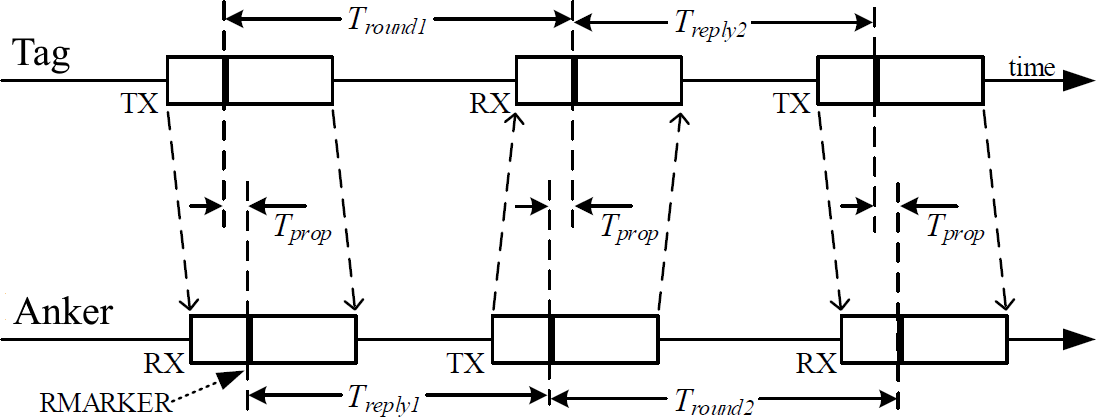
\includegraphics[width=0.70\linewidth]{double_sided_two_way_ranging}
	\caption{Ablauf des \acrlong{dstwr}.}
	\source{\citetitle{decawave2016dw1kusermanual} \cite{decawave2016dw1kusermanual}}
	\label{fig:double_sided_two_way_ranging}
\end{figure}

Die ungefähre \Gls{tof}--Zeitspanne ergibt sich aus der folgenden Gleichung:

\[T_{prop}=\frac{\left(T_{round1}\times T_{round2}-T_{reply1}\times T_{reply2}\right)}{\left(T_{round1}+T_{round2}+T_{reply1}+T_{reply2}\right)}\]

Der Fehler bei diesem Verfahren ergibt sich aus der folgenden Gleichung:

\[error=T_{prop}\times\left(1-\frac{k_a+k_b}{2}\right)\] 

Die Variablen $k_a$ und $k_b$ entsprechen hierbei den Offsetfehler der Zeitgeber von der Nennfrequenz und liegen beide sehr nahe bei eins.

Mit diesem Verfahren ist es auch möglich, gleichzeitig die Entfernungen zu mehr als einem \Gls{anchor} zu bestimmen, siehe \figurename~\ref{fig:double_sided_two_way_ranging_with_three_anchor}. Hierbei weist der \Gls{tag} in der initialen Nachricht jedem \Gls{anchor} eine individuelle Antwortzeit zu. Danach wartet er bist alle Antwortnachrichten angekommen sind um im der letzten Nachricht, dann jedem \Gls{anchor} seine Umlauf-- und Antwortzeiten zu übermitteln. Jeder \Gls{anchor} kann nun individuell die \Gls{tof}--Zeitspanne für sich berechnen und dann dem \Gls{tag} übermitteln. Diese letzte Nachricht ist auf der \figurename~\ref{fig:double_sided_two_way_ranging_with_three_anchor} nicht aufgeführt.

\begin{figure}[ht]
	\centering
	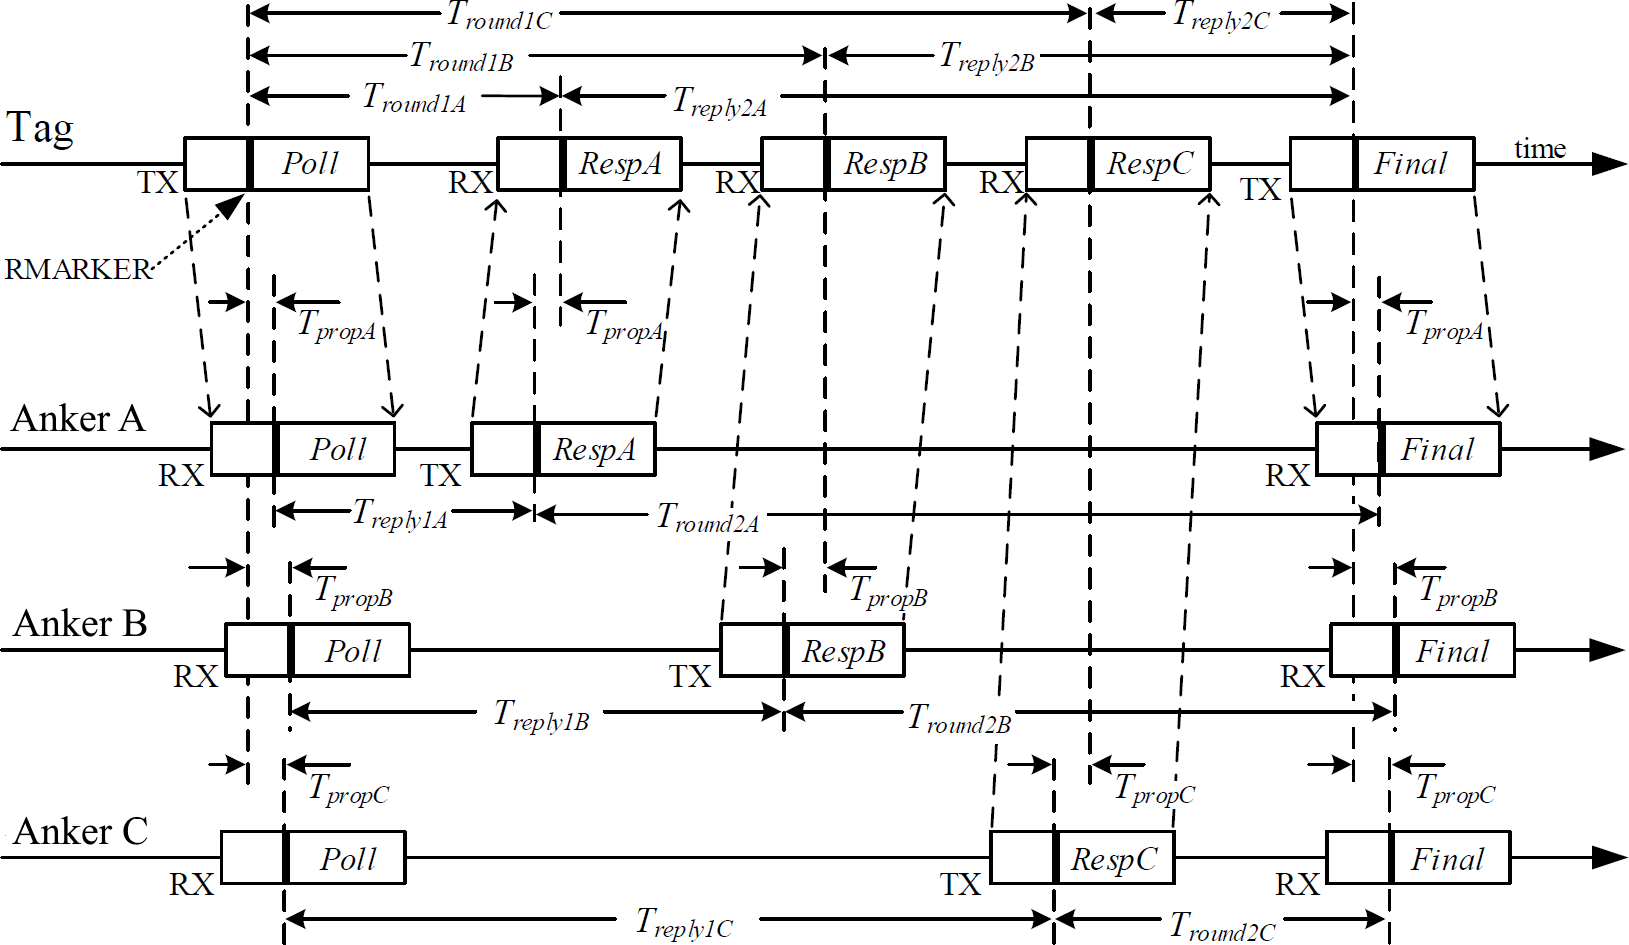
\includegraphics[width=0.8\linewidth]{double_sided_two_way_ranging_with_three_anchor}
	\caption{Ablauf des \acrlong{dstwr} mit einem \Gls{tag} und drei \Gls{anchor}.}
	\source{\citetitle{decawave2016dw1kusermanual} \cite{decawave2016dw1kusermanual}}
	\label{fig:double_sided_two_way_ranging_with_three_anchor}
\end{figure}

In der \figurename~\ref{fig:double_sided_two_way_ranging_with_three_anchor} wurde in der initialen Nachricht jedem \Gls{anchor} eine individuelle Antwortzeit zugeordnet. Woher wusste der\Gls{tag} welche \Gls{anchor} vorhanden sind? Die Kommunikation zwischen \Gls{tag} und \Gls{anchor} kann in zwei Phasen unterteilt werden, siehe \figurename~\ref{fig:discovery_and_ranging_phase}. In der \textit{Discovery} Phase schickt der \Gls{tag} periodisch \textit{Blink} Nachrichten mit seiner Identifikationsnummer an alle Module in der Umgebung. Empfängt ein \Gls{anchor} diese Nachricht, nimmt er den \Gls{tag} in seiner Liste auf und übermittelt dem \Gls{tag} eine \textit{Ranging Init} Nachricht mit seiner Identifikationsnummer. Das \Gls{tag} seinerseits nimmt den \Gls{anchor} in seiner Liste auf und weiß nun auch welche \Gls{anchor} er in der nächsten Entfernungsmessung berücksichtigen muss. Die \textit{Ranging} Phase entspricht hierbei der bereits zuvor besprochenen Entfernungsmessung.

\begin{figure}[ht]
	\centering
	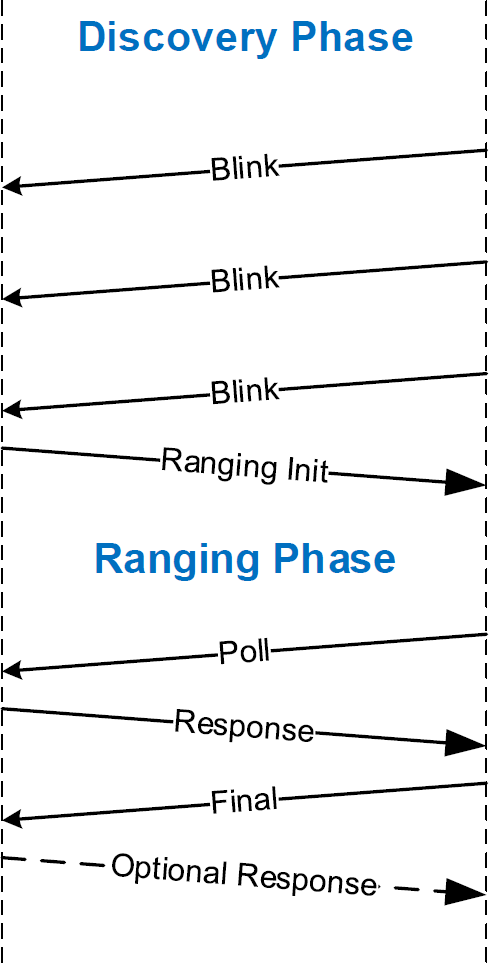
\includegraphics[width=0.40\linewidth]{discovery_and_ranging_phase}
	\caption{Ablauf der \textit{Discovery} und \textit{Range Phase} zwischen einem \Gls{tag} und mehreren \Gls{anchor}n.}
	\source{\citetitle{decawave2016dw1kusermanual} \cite{decawave2016dw1kusermanual}}
	\label{fig:discovery_and_ranging_phase}
\end{figure}


\begin{comment}
------------------------------------------------------------------------------------------
\end{comment}
\section{Geometrie}


\begin{comment}
------------------------------------------------------------------------------------------
\end{comment}
\subsection{Gleichseitiges Dreieck}

Ein gleichseitiges Dreieck zeichnet sich dadurch aus, dass alle drei Seiten gleich lang sind und jeder Innenwinkel einen Wert von \SI{60}{\degree} besitzt, siehe \autoref{fig:wikipedia_gleichseitiges_dreieck}. Ist der Umkreisradius $r_u$ eines gleichseitigen Dreiecks bekannt, so kann mit der \autoref{eq:dreieck_seitenlaenge_aus_umkreis} auch die Seitenlänge $a$ berechnet werden.

\begin{equation}
a = \frac{3}{\sqrt{3}} r_u \label{eq:dreieck_seitenlaenge_aus_umkreis}
\end{equation}


\begin{comment}
------------------------------------------------------------------------------------------
\end{comment}
\subsection{Regelmäßiges Fünfeck}

Das regelmäßige Fünfeck zeichnet sich dadurch aus, das alle fünf äußeren Seiten gleich lang sind und jeder Innenwinkel einen von Wert von \SI{108}{\degree} besitzt, siehe \autoref{fig:wikipedia_regelmaessiges_fuenfeck}. Aus der Länge einer äußeren Seite $a$ lässt sich zum einen der Umkreisradius $r_u$, siehe \autoref{eq:fuenfeck_umkreisradius}, und die Diagonale $d$ zwischen zwei Spitzen, siehe \autoref{eq:fuenfeck_diagonale}, berechnen.

\begin{equation}
r_u = \frac{a}{10} \sqrt{50 + 10 \sqrt{5}} \label{eq:fuenfeck_umkreisradius}
\end{equation}

\begin{equation}
d = \frac{a}{2} \left(1 + \sqrt{5} \right) \label{eq:fuenfeck_diagonale}
\end{equation}


\begin{comment}
------------------------------------------------------------------------------------------
- Theorie: Wahrscheinlichkeitsverfahren
	- Positionsschätzer in Form einer Wahrscheinlichkeitsverteilung über den Zustandraum.
	- Kalman fitering
		- Multivariate Gaussian distribution (Mehrdimensionale Normalverteilung)
		- \url{https://de.wikipedia.org/wiki/Mehrdimensionale_Normalverteilung}
		- Kompakte Beschreibung der Normalverteilung über den Erwartungswert $\mu$ und die Kovarianzmatrix $\Sigma$ ($\mu$ und $\sigma^2$)
		- \url{https://matheguru.com/stochastik/normalverteilung.html}
	- Markov methods
		- Probability Grid
		- Robot--Position ist diskretisiert
		- Nutzen von Bayes Rule um Grids zu kombinieren/neuerzeugen
	- Monte Carlo Lokalisierung
		- Multimodal Distribution for position estimation
		- Important Sampling
- http://www.mathepedia.de/Stochastik.html
- Zufallsvariable, Massenfunktion, Dichtefunktion und Verteilungsfunktion
	- https://www.youtube.com/watch?v=DoHTsDrzAQk
- Introduction to Mobile Robotics - SS 2017
	- http://ais.informatik.uni-freiburg.de/teaching/ss17/robotics/
- https://en.wikipedia.org/wiki/Conditional_dependence
- https://www.mrpt.org/tutorials/slam-algorithms/rangeonly_slam/


- A modern introduction to probability and statistics.pdf
- Introduction_to_Kalman_Filtering.pdf

- Bayesian statistics
	- https://en.wikipedia.org/wiki/Bayesian_statistics
	- Law of total probability
		- https://en.wikipedia.org/wiki/Law_of_total_probability
- Rule of Total Probability and Bayes' Rule
	- https://www.youtube.com/watch?v=VvThd5zRQC4
	- https://www.youtube.com/watch?v=8SCmdX68pIk
	
- Robot Mapping - WS 2016/17 - Uni-Freiburg
	- http://ais.informatik.uni-freiburg.de/teaching/ws16/mapping/
	- https://www.youtube.com/playlist?list=PLgnQpQtFTOGQrZ4O5QzbIHgl3b1JHimN_&feature=g-list
	
- Probabilistic Robotics
	- http://robots.stanford.edu/probabilistic-robotics/


\end{comment}


\begin{comment}
------------------------------------------------------------------------------------------
State = Zustand
Environment = Umwelt
Percept = Wahrnehmnung
Control Action = Steuerbefehle
\end{comment}
\section{Zustände}

Ein Roboter der sich in seiner Umwelt zurechtfinden soll, muss diese modellieren. Das Ergebnis der Modellierung bezeichnet man als Zustand. Ein Zustand beschreibt dabei alle Aspekte des Roboters und seiner Umwelt die einen Einfluss auf die Zukunft haben können. Ein Zustand kann dabei aus statischen sowie dynamischen Komponenten bestehen. Aus dem letzteren ergibt sich zwangsweise, dass ein Zustand sich auch über die Zeit verändern kann. Ein Zustand kann z.B. die Pose des Roboters sein, die Positionen von stationären Landmarken oder aber auch der Ladezustand der Energieversorgung. Beschrieben wird er Zustand mit dem Symbol $x$.

% todo: What is a complete state?

Die meisten Roboter verfügen über Sensoren um Änderungen an Ihrer Umwelt wahrzunehmen. Diese Wahrnehmungen werden dabei mit dem Symbol $z$ beschrieben. Zusätzlich kann der Roboter aktiv Änderungen an seiner Umwelt vornehmen, in dem er Steuerbefehle and die Aktorik sendet und sich somit durch seine Umwelt bewegt. Steuerbefehle werden mit dem Symbol $u$ beschrieben.

Um Auszudrücken, dass die Information des Zustandes, der Wahrnehmung und der Steuerbefehle, zu einem bestimmen Zeitpunkt gehören wird der Index $x_t$ verwendet. Eine Zeitspanne wird über den Index $x_{1:t}$ ausgedrückt. Im mathematischen Sinne werden alle drei Größe als Spaltenvektoren beschrieben, die nicht über die gleiche Dimension verfügen müssen. Zum Beispiel könnte der Zustand aus den X-/Y-Position und der Orientierung $\theta$ zusammengesetzt sein, während die Wahrnehmung aus vielen hunderten Entfernungsmessungen bestehen.


\begin{comment}
------------------------------------------------------------------------------------------
\end{comment}
\section{Wahrscheinlichkeitstheorie}

In der Theorie kann der Zustand eindeutig bestimmt werden, in der Praxis ist dieser nicht mehr so eindeutig. Um diese Unsicherheit abzubilden, wird in der Robotik die Wahrscheinlichkeitstheorie angewendet. Dabei wird der Zustand als eine kontinuierliche Zufallsvariable angesehen. Ob sich nun ein System in einem bestimmten Zustand befindet, wird über eine \Gls{wdf} beschrieben. In der Regel wird eine gaußsche Normalverteilung eingesetzt, die sich über den Mittelwert $\mu$ und Varianz $\sigma^2$ beschreiben lässt, siehe \autoref{eq:normal_distribution}. Häufig wird die Normalverteilung auch über $\operatorname{\mathcal{N}}{(x; \mu, \sigma^2)}$ abgekürzt.

\begin{equation}
p(x) = \left( 2 \pi \sigma^2 \right)^{-\frac12}  \exp{ \left\{ -\frac12 \frac{(x - \mu)^2}{\sigma^2} \right\} } \label{eq:normal_distribution}
\end{equation}

Da es sich bei dem Zustand nicht um einen skalaren Wert handelt, muss eine mehrdimensionale Normalverteilung eingesetzt werden, siehe \autoref{eq:multivariate_normal_distribution}. Diese wird über einen Vektor der Mittelwert $\mu$ und eine symmetische Kovarianzmatrix $\Sigma$ beschrieben.

\begin{equation}
p(x) = \operatorname{det}{\left( 2 \pi \Sigma \right)}^{-\frac12}  \exp{ \left\{ -\frac12 (x - \mu)^T \Sigma^{-1} (x - \mu) \right\} } \label{eq:multivariate_normal_distribution}
\end{equation}

Die Multivariate Verteilung zweier Zufallsvariablen beschreibt die Wahrscheinlichkeit, mit welcher das Ereignis $x$ sowie das Ereignis $y$ auftritt. Sollen beide Zufallsvariablen unabhängig von einander sein, so lassen sich ihre Wahrscheinlichkeiten multiplizieren, siehe \autoref{eq:independent_joint_distribution}.

\begin{equation}
p(x, y) = p(x) \, p(y) \label{eq:independent_joint_distribution}
\end{equation}

Von der bedingten Wahrscheinlichkeit spricht man dann, wenn eine Zufallsvariable, Wissen über eine anderen Zufallsvariable besitzt, siehe \autoref{eq:conditional_probability}.

\begin{equation}
p(x \mid y) = \frac{p(x, y)}{p(y)} \label{eq:conditional_probability}
\end{equation}

Die bedingte Wahrscheinlichkeit von zwei Zufallsvariablen die unabhängig von einander sind, reduzieren sich zu der Wahrscheinlichkeit einer Zufallsvariable, siehe \autoref{eq:independent_joint_distribution} und \autoref{eq:independent_conditional_probability}.

\begin{equation}
p(x \mid y) = \frac{p(x) \, p(y)}{p(y)} = p(x) \label{eq:independent_conditional_probability}
\end{equation}

Der Satz von Bayes sagt aus, das ein Verhältnis zwischen der bedingten Wahrscheinlichkeit $p(x \mid y)$ und der umgekehrten Form $p(y \mid x)$ besteht, siehe \autoref{eq:bayes_rule}.

\begin{equation}
p(x \mid y) = \frac{p(y \mid x) \, p(x)}{p(y)} \label{eq:bayes_rule}
\end{equation}

Der Nenner $p(y)$ hängt nicht von $x$ ab, ist daher für jedes Ereignis konstant und wird als Konstante $\eta$ vor die Gleichung gesetzt, siehe \autoref{eq:bayes_rule_with_normalizer}.

\begin{equation}
p(x \mid y) = \eta \, p(y \mid x) \, p(x) \label{eq:bayes_rule_with_normalizer}
\end{equation}


\begin{comment}
------------------------------------------------------------------------------------------
- https://matheguru.com/stochastik/standardfehler.html
- https://de.wikipedia.org/wiki/Standardfehler
- Theorie: Lokalisierungsprobleme
	- Statische Lokalisierung
		- Akkurate Schätzung seiner globalen Position anhand der Sensordaten
		- Annahme: Umgebungskarte der Landmarken ist vorhanden
	- Position Tracking/Positionsverfolgung
		- Initiale Position ist gegeben
		- Verfogenden der Roboterposition
		- Annahme: Umgebungskarte der Landmarken ist vorhanden
	- SLAM
		- Verwenden der Sensordaten um sich zu Lokalisierung...
		- und eine Karte der Landmarken zu erzeugen.
		- Bisher Winkel und Entferung zu einer Landmarke gegeben
			- Computer Vision, Structure from Motion
		- Hier nur die Entfernung
- A Short Introduction to the Bayes Filter and Related Models
	- http://ais.informatik.uni-freiburg.de/teaching/ws12/mapping/pdf/slam02-bayes-filter-short.pdf
- Bayes Filter
	- https://www.tu-chemnitz.de/informatik/KI/edu/robotik/ws2012/robotik_6_2.pdf
\end{comment}
\section{Bayes Filter}


\begin{equation}
\operatorname{bel}{x_t} = p(x_t \mid z_{1:t}, u_{1:t}) \label{eq:bayes_filter_prediction}
\end{equation}

\begin{equation}
\overline{\operatorname{bel}{p(x_t \mid z_{1:t-1}, u_{1:t})}} \label{eq:bayes_filter_correction}
\end{equation}



\begin{comment}
------------------------------------------------------------------------------------------
- \cite{kalman1960new}
- \cite{kurth2003experimental}
	- Originally introduced in 1960, the Kalman Filter assumes a multivariate Gaussian distribution [6]. The Kalman Filter has the advantage that the representation of the distribution is compact; a Gaussian distribution can be represented by a mean and a covariance matrix. The robot's pose estimation is maintained as a Gaussian distribution and sensor data from dead reckoning and landmark observations is fused to obtain a new position distribution.
	- Our results with Kalman Filtering require an under-standing of the characteristics of the noise present in ranges reported by the radio tags. We gain this by look-ing at the probability distribution functions for each tag measurement.
	- We obtain the PDFs as follows: for every reported measurement, we and the true range to the robot when that distance was reported. We do this by comparing the known location of the reporting tag to the times-tamped true location of the robot when the report was received.
	- the covariance matrix, which describes the uncertainty and correlation of the terms in the state estimate.
	- However, when the same initial noisy tag locations are used with Test 2, our SLAM technique fails to converge. Since the Kalman Filter uses a linearization of the nonlinear range measurements, if the linearized estimate is too far away from the truth, the Filter may be unable to recover and will diverge.

- https://www.youtube.com/watch?v=CaCcOwJPytQ
	- Special Topics - The Kalman Filter (1 of 55) What is a Kalman Filter?

\end{comment}
\subsection{Kalman Filter [todo]}


\begin{comment}
------------------------------------------------------------------------------------------
- \cite{kurth2003experimental}
	- Recent extensions of Kalman Filtering allow for non-Gaussian, multimodal probability distributions through multiple hypothesis tracking. The result is a more versatile estimation technique that still preserves many of the computational advantages of the Kalman filter.
\end{comment}
\subsection{Extended Kalman Filter [todo]}

% Linearisierung, 


\begin{comment}
------------------------------------------------------------------------------------------
\end{comment}
\section{Partikel Filter [todo]}

\begin{comment}
------------------------------------------------------------------------------------------
- \cite{kurth2003experimental}
	- Monte Carlo localization, or particle filtering, provides a method of representing multimodal distri-butions for position estimation [4, 12], with the ad-vantage that the computational requirements can be scaled. The main advantage of these methods is their ability to recover robustly from a poor initial condition.
- \cite{fox1999monte}
\end{comment}
\subsection{Monte Carlo [todo]}


\begin{comment}
------------------------------------------------------------------------------------------
Rao-Blackwellized Particle Filtering
https://people.eecs.berkeley.edu/~pabbeel/cs287-fa12/slides/RBPF.pdf

- \cite{murphy2001rao}
	- Rao-Blackwellised particle filtering for dynamic Bayesian networks
\end{comment}
\subsection{Rao-Blackwellized [todo]}


\begin{comment}
------------------------------------------------------------------------------------------
- \cite{kurth2003experimental}
	- We are currently developing a batch localization method, which considers all the data collected by the robot and finds the best path estimate given all the data. Although time consuming computationally, this will produce the theoretically optimal result obtainable from the collected data; we can then evaluate the results of our online localization method by comparing to this optimal solution.
- \cite{}
	- Comparison of Batch and Kalman Filtering for Radar Tracking
	- http://www.dtic.mil/dtic/tr/fulltext/u2/p011192.pdf
	- The EKF propagates the filter state between measurements, and incorporates measurements sequentially, with the error dynamics and observation models respectively. It is an implementation of the often referenced linear-minimum-variance (Kalman) formulas, adapted by first-variation approximations of the nonlinear models, centered at the current state estimate, and described in Reference [4] (Jazwinski). 	
	- The Batch algorithm, in comparison, processes those same measurements simultaneously via iterative least-squares estimation. An overview of the comparison of measurement processing among the two algorithms is shown in Figure-1. Batch algorithm estimations were made in parallel with those of the EKF for comparison of estimation error time histories.
\end{comment}
%\section{Batch optimization [todo,optional]}


\begin{comment}
------------------------------------------------------------------------------------------
- \cite{kurth2003experimental}
	- Additionally, we will extend the batch method to produce a variable dimension filter, as used by Deans for the case of bearing-only sensors [3], which would consider some window of previous robot states and optimize the position estimates based on the data in that window.
\end{comment}
%\section{Variable Dimension Filter [todo,optional]}


\begin{comment}
------------------------------------------------------------------------------------------
Embodied Localisation and Mapping
http://elib.suub.uni-bremen.de/edocs/00103537-1.pdf

"C:\Users\Albert\Documents\Studium\Bachelor WS17\scientific publication\Efficient probabilistic range-only SLAM.ppt"


- \citez{montemerlo2002fastslam}
	- FastSLAM: A factored solution to the simultaneous localization and mapping problem

- \cite{sarkka2013bayesian}
	- Bayesian filtering and smoothing
- \cite{kurth2003experimental}
	- The Kalman Filter approach described in Section 5 can be reformulated for the SLAM problem. To perform SLAM, we include position estimates for each tag in the state, producing a state vector of the form: q(k) = [xk; yk; k; xb1; yb1 ; :::; xbn; ybn]T , where n is the number of beacons.
	
- The purpose of a probabilistic approach to RO-SLAM is to obtain the joint probability distribution of the robot pose (or path) and the map, given all the available data at some instant of time. This distribution represents our knowledge about the robot path, the map, and all their correlations.
\end{comment}
\section{SLAM [todo]}

% Zuerst wird die Position geschätzt und danach die Positionen der Landmarken.

\begin{comment}
------------------------------------------------------------------------------------------
\end{comment}
\subsection{RO--SLAM [todo]}


\begin{comment}
------------------------------------------------------------------------------------------
- \url{https://www.heise.de/developer/artikel/Einfuehrung-in-das-Robot-Operating-System-3273655.html?seite=all}
- Node = Knoten
- Topic = Datenbus
- Service = Dienst
- Message = Nachricht
- Launch-Files = Startdateien
\end{comment}
\section{Robot Operating System}

Bei dem \Gls{ros} handelt es sich nicht im eigentlichen Sinne um ein Betriebssystem, sondern vielmehr um ein Framework das die Kommunikation zwischen verschiedenen Verarbeitungseinheiten regelt. Im Jahre 2007 begann die Entwicklung von \Gls{ros} an der Stanford University. Ab 2009 wurde dieses dann hauptsächlich an dem Robotik Institut Willow Garage weiterentwickelt. Durch die BSD Lizenz steht \Gls{ros} als Open--Source--Projekt sowohl der nicht--kommerziellen auch der kommerziellen Weiterentwicklung zur Verfügung. \cite{quigley2009ros}

Jedes \Gls{ros}--System muss über einen \Gls{ros}--Master verfügen. Dieser stellt den zentralen Punkt für die Registrierung von Knoten (engl. Nodes), Datenbusse (engl Topics) und Dienste (engl. Services) zur Verfügung.

Jeder Verarbeitungseinheit in \Gls{ros} wird durch einen Knoten repräsentiert. Ziel ist es möglichst kleine, wiederverwendbare und miteinander kombinierbare Einheiten zu bilden. Die Programmierung eines Knoten erfolgt dabei in den Programmiersprachen C++, Python oder Lisp.

Die Kommunikation zwischen den Knoten erfolgt dabei über ein \Gls{p2p}--Kanal auf der Basis von Nachrichten (engl. Messages). Bei einer Nachricht handelt es sich um eine Datenstruktur die primitive Datentypen, die Datentypstruktur anderer Nachrichten und Felder enthalten kann. Eine Nachricht wird dabei über das \textit{Publish--Subscribe} Muster in einem Datenbus veröffentlicht und kann von jedem Knoten empfangen werden der Nachrichten von diesem Datenbus abonniert hat. Der typische Anwendungsfall für dieses Verfahren ist die Bereitstellung von Sensordaten und Rückmeldungen über Statusänderungen.

Das zuvor vorgestellte \textit{Publish--Subscribe} Muster stellt eine asynchrone Kommunikation bereit. Mit Hilfe von Diensten ist auch ein synchroner Nachrichtenaustausch möglich. Hierfür wird eine Anfrage von dem \textit{Client} an den \textit{Server} gestellt, der seinerseits mit einem Ergebnis antwortet. Dieses Verfahren entspricht dem \textit{Request--Response} Muster. Die Erstellung einer inversen Transformation ist ein typischer Anwendungsfall hierfür.

Nach der Entwicklung neuer Algorithmen ist ein Vergleich mit den bereits bestehenden Algorithmen von großem Interesse. Mit dem Konzept der \textit{Bag}--Dateien können alle veröffentlichten Nachrichten aufgezeichnet werden und zu einem späteren Zeitpunkt wieder abgespielt werden.

Um die Wiederverwendbarkeit von Knoten, Nachrichten und Diensten zu fördern, wurde das Konzept der Pakete (engl. Packages) eingeführt. Ein Paket stellt die kleinste erstellbare Einheit dar und beinhaltet alle Teile eines Softwarepaketes wie z.B. Quellcode--, Konfigurationsdateien, Drittanbieter Bibliothek, Abhängigkeitslisten usw.

Eine Roboterplattform besteht aus vielen Sensoren und Aktuatoren die abgefragt und gesteuert werden müssen. Dementsprechend viele Knoten müssen gestartet werden. Diese Aufgabe erfüllen die Startdateien (engl. Launch-Files). Neben der Definition der Knoten die gestartet werden sollen, können Einzelne oder eine Gruppe von Knoten parametrisiert werden. Mittels der Verschachtelung von Startdateien ist eine Wiederverwendung von knotenspezifischen Startdateien möglich.

Zu den häufigsten Operationen der Verarbeitungseinheit einer Roboterplattform ist das Transformieren der Sensordaten aus dem Sensorkoordinatensystem in das Koordinatensystem des Robotermittelpunktes. In \Gls{ros} wird hier für ein Transformationsbaum (engl. TF--Tree) verwendet, der aus statischen und dynamischen Transformationen besteht. Statische Transformationen werden dort eingesetzt, wo sich die Pose zweier Koordinatensysteme zur Laufzeit nicht ändert, z.B. zwischen dem Robotermittelpunkt und einem fest montierten Sensor. Dynamische hingegen bei Koordinatensystemen die sich zur Laufzeit ändern, z.B. zwischen dem Robotermittelpunkt und den Inkrementalgebern der Antriebseinheit. Statische Transformationen können mittels einer URDF--Datei modelliert und allen Knoten bereitgestellt werden.

